\chapter{Evaluation}
\label{ch:Evaluation}

This chapter provides information about the input data acquired from different sources, the methods that were used to forecast electricity load and other statistical methods and also evaluates them regarding performance and the quality of the output.\\
%In this chapter, the used methods will be evaluated and critically regarded considering their performance and the quality of their outputs.\\

\section{Data}
\label{sec:data}

%Of course choosing data sources as well as sorting and cleaning the data also requires a certain amount of time and effort. Thus it will be explained hereinafter how this has been done for the data used in this thesis.

\subsection{ECMWF}

The data used in this thesis originates from \acrshort{ecmwf}, which is a research institute that produces global numerical weather predictions and other data.\\
It is time series based and for each timestamp there is a 2-dimensional array referred to by longitude and latitude respectively.\\

It must be mentioned that, as the data used has been reanalysed, so the expected error is likely to be smaller than if working with real-time data.\\

As data parameters there are also longitude and latitude, where the longitude is chosen to be from 5.5 to 15.5 and the latitude from 47 to 55.5. As the resolution of the used grid is at 0.25°, this results in a total of 1435 grid points per timestamp. As the range of the data from \acrshort{ecmwf} extends from 2015/1/1 to 2019/3/31(TODO update), there is a total of 1551 days with each 12 timestamps due to the 2 hours frequency and thus 18612 timestamps. Considering that there is a value for each point in the grid and every timestamp, there are 26708220 values for each variable.\\

Plotting the data on a map results in a result as can be seen in \Cref{fig:maxvar4_maps} and \Cref{fig:isin_compare}. In this case the temperature measured at 2 metres is visualized.\\

%\begin{figure}[h!]%
%\centering
%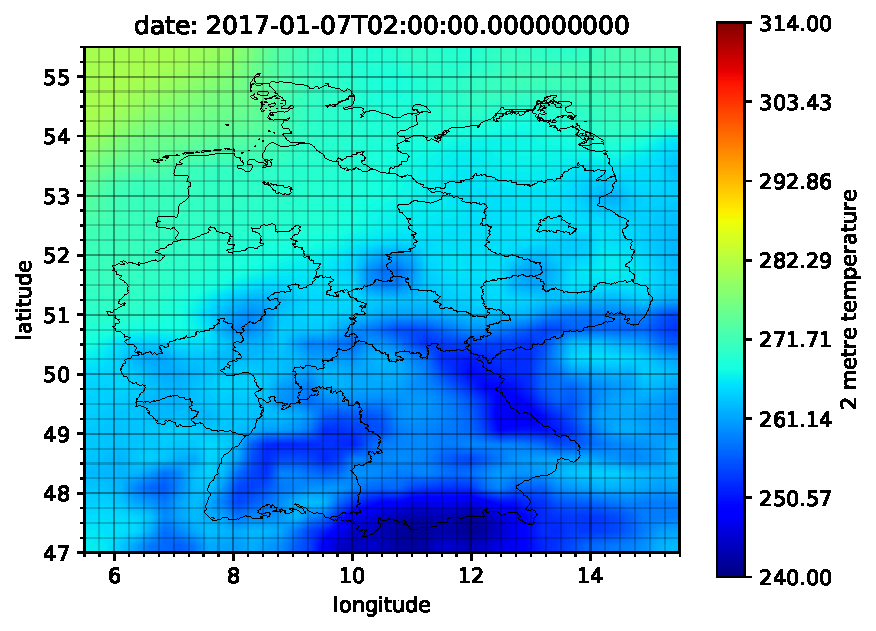
\includegraphics[width=\textwidth]{plots/0_2017010702_20190617161317}%
%\caption{Map showing day with lowest temperature in germany.}%
%\label{fig:0_2017010702_20190617161317}%
%\end{figure}

\begin{figure}[h!]%
\centering
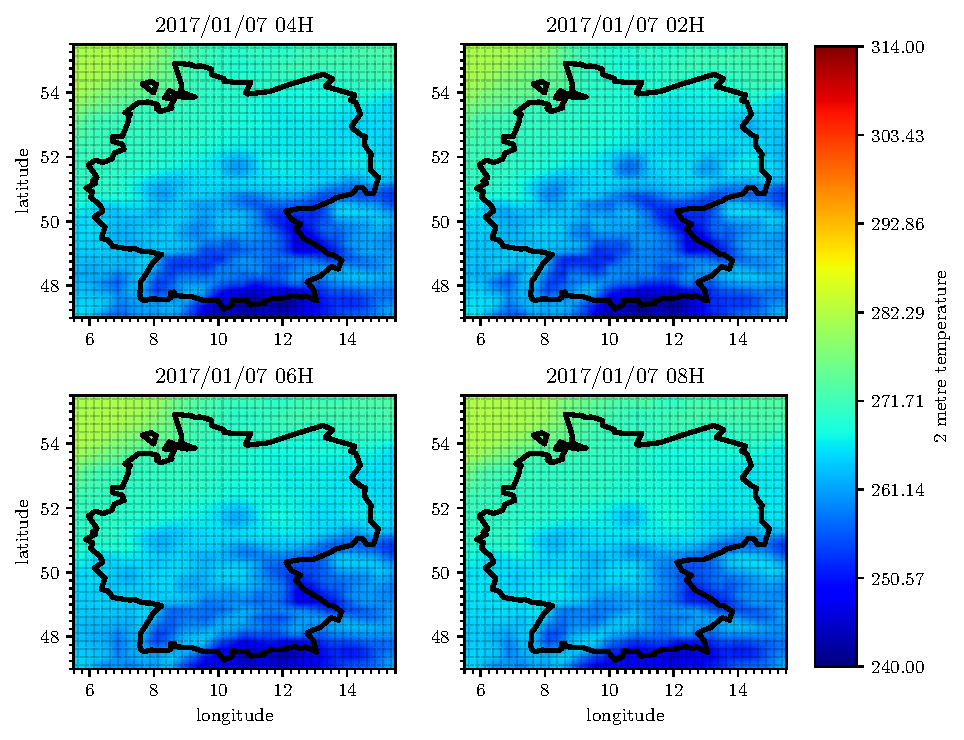
\includegraphics[width=\textwidth]{plots/t2m/bundles/maxvar4_maps}%
\caption{Four maps showing the four times with the highest two metre temperature variance in Germany, where top left is the highest, top right the second highest, bottom left the third highest and bottom right the fourth highest variance.}%
\label{fig:maxvar4_maps}%
\end{figure}

In order to reduce complexity, a shapefile of the \acrshort{nuts} dataset was used. The shapefile contains all countries in the EU. The shape of Germany was filtered from this data and each point in the dataset is checked whether it is within Germany or not. The result can be seen in \Cref{fig:isinDE}. The filtered map first is saved in a numpy.ndarray and then applied on the data to mask unwanted data visualized in \Cref{fig:t2m_maxvar_0_map_isin}.\\

\begin{figure}[h!]%
	\centering
	\begin{subfigure}{.5\textwidth}
		\centering
		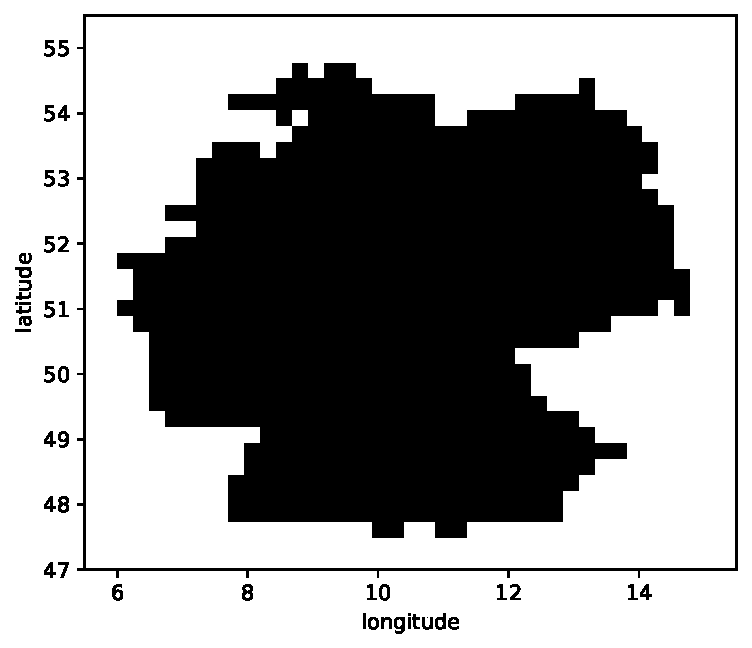
\includegraphics[width=.85\textwidth]{plots/isinDE}%
		\label{fig:isinDE}%
	\end{subfigure}%
	\begin{subfigure}{.5\textwidth}
		\centering
		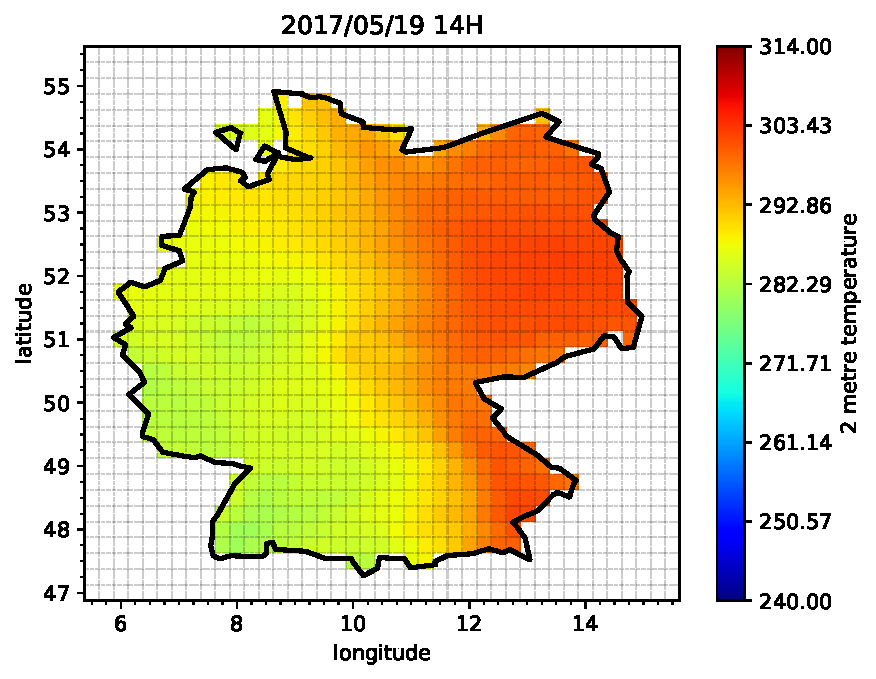
\includegraphics[width=1.1\textwidth]{plots/t2m/maxvar/0_map_isin}%
		\label{fig:t2m_maxvar_0_map_isin}%
	\end{subfigure}
	\caption[2D boolean numpy.ndarray (left) used to filter grid squares that are within Germany. It was created by using a shapefile of Germany from Eurostat and checking for each point of the grid if it is within the shapefile. When applied to the weather data, only relevant data within Germany is obtained (right).]
	{2D boolean numpy.ndarray (left) used to filter grid squares that are within germany. It was created by using a shapefile of Germany from Eurostat\footnotemark and checking for each point of the grid whether it is within the shape. When applied to the weather data, only relevant data within Germany is obtained (right).}
	\label{fig:isin_compare}
\end{figure}
\footnotetext{\url{https://ec.europa.eu/eurostat/de/web/gisco/geodata/reference-data/administrative-units-statistical-units/nuts}}

The initial dataset contains a set of variables listed in \Cref{tab:wvars} where also the units, min and max are shown for each variable respectively.\\

\begin{table}[h!]%
\rowcolors{2}{white}{gray!25}
\centering
\footnotesize
\begin{tabularx}{\linewidth}{Llrr}
\tablehead variable name & \tablehead units & \tablehead min & \tablehead max \\\hline
10 metre U wind component & $m~s^{-1}$ & -18.56 & 21.92 \\
10 metre V wind component & $m~s^{-1}$ & -21.51 & 20.00 \\
2 metre temperature & $K$ & 240.97 & 313.26 \\
Leaf area index, high vegetation & $m^{2}~m^{-2}$ & 0.00 & 4.90 \\
Leaf area index, low vegetation & $m^{2}~m^{-2}$ & 0.00 & 3.84 \\
Low cloud cover & $(0~-~1)$ & 0.00 & 1.00 \\
Soil temperature level 1 & $K$ & 257.91 & 313.64 \\
Surface latent heat flux & $J~m^{-2}$ & -2203977.00 & 359411.00 \\
Surface net thermal radiation & $J~m^{-2}$ & -663417.00 & 142945.02 \\
Surface sensible heat flux & $J~m^{-2}$ & -1703159.00 & 801354.00 \\
Total cloud cover & $(0~-~1)$ & 0.00 & 1.00 \\
Total column rain water & $kg~m^{-2}$ & 0.00 & 2.73 \\
Total sky direct solar radiation at surface & $J~m^{-2}$ & -0.12 & 3088320.00 \\
\end{tabularx}
\caption[List of exogenous weather variables used to forecast the load including min, max values from \acrshort{ecmwf}.]{List of exogenous weather variables used to forecast the load including min, max values from \acrshort{ecmwf}\footnotemark.}
\label{tab:wvars}
\end{table}
\footnotetext{\url{https://www.ecmwf.int/en/forecasts/datasets/browse-reanalysis-datasets}}


\subsection{Load data}

Besides weather data used to refine the forecasting results, also historic load data was needed. Therefore data has been retained from Open Power System Data\footnote{\url{https://data.open-power-system-data.org/time_series/}}. \Cref{fig:t2m_mean_2015010112_2018123112_24F} shows the distribution of loads over time with one point per day at 12 am UTC time. The color shows the mean temperature measured at 2 metres.\\

%\begin{figure}[h!]%
%\centering
%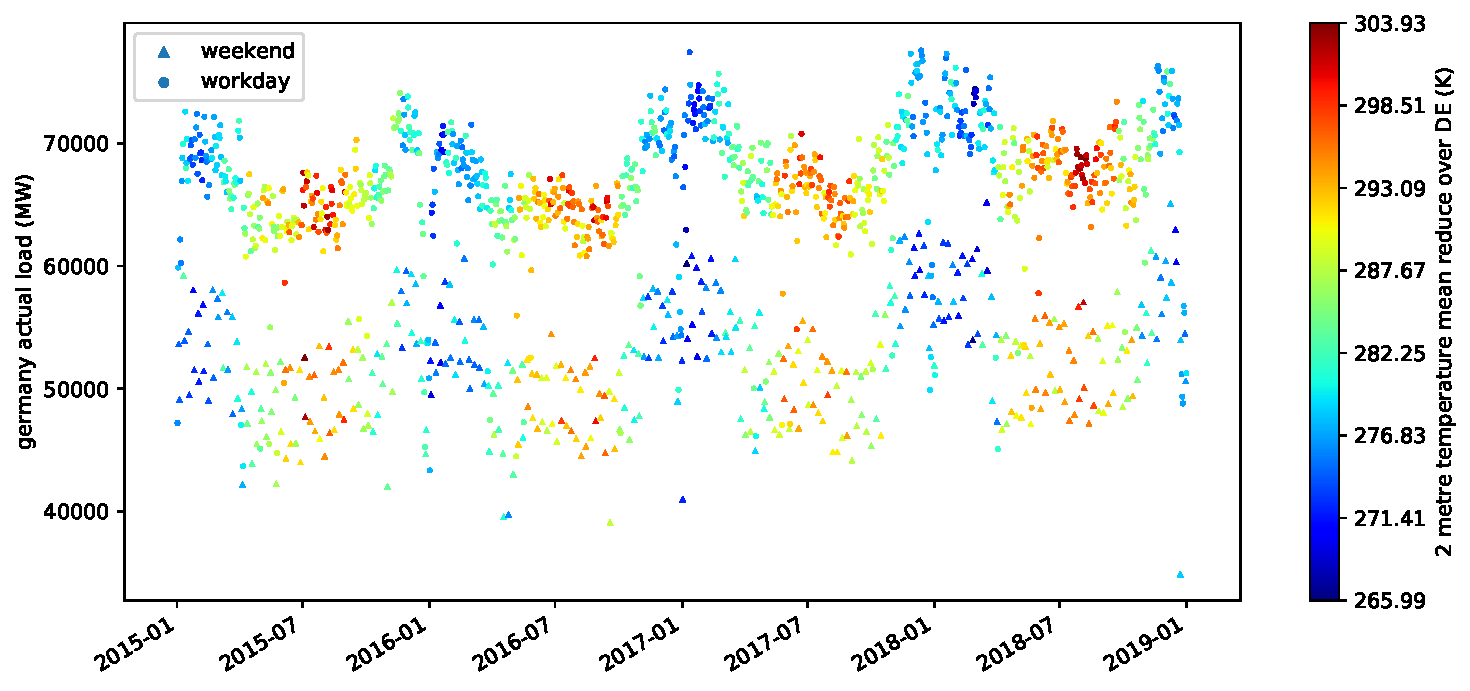
\includegraphics[width=\textheight,angle=-90,origin=c]{plots/t2m_mean_2015010112_2018123112_24F}%
%\caption{Load curve with mean of 2 metre height measured temperature in germany as color from 2015/1/1 to 2018/12/31 with one single point per day at 12am utc time respectively.}%
%\label{fig:t2m_mean_2015010112_2018123112_24F}%
%\end{figure}

\begin{figure}[H]%
	\centering
	\begin{subfigure}{.5\textwidth}
		\centering
		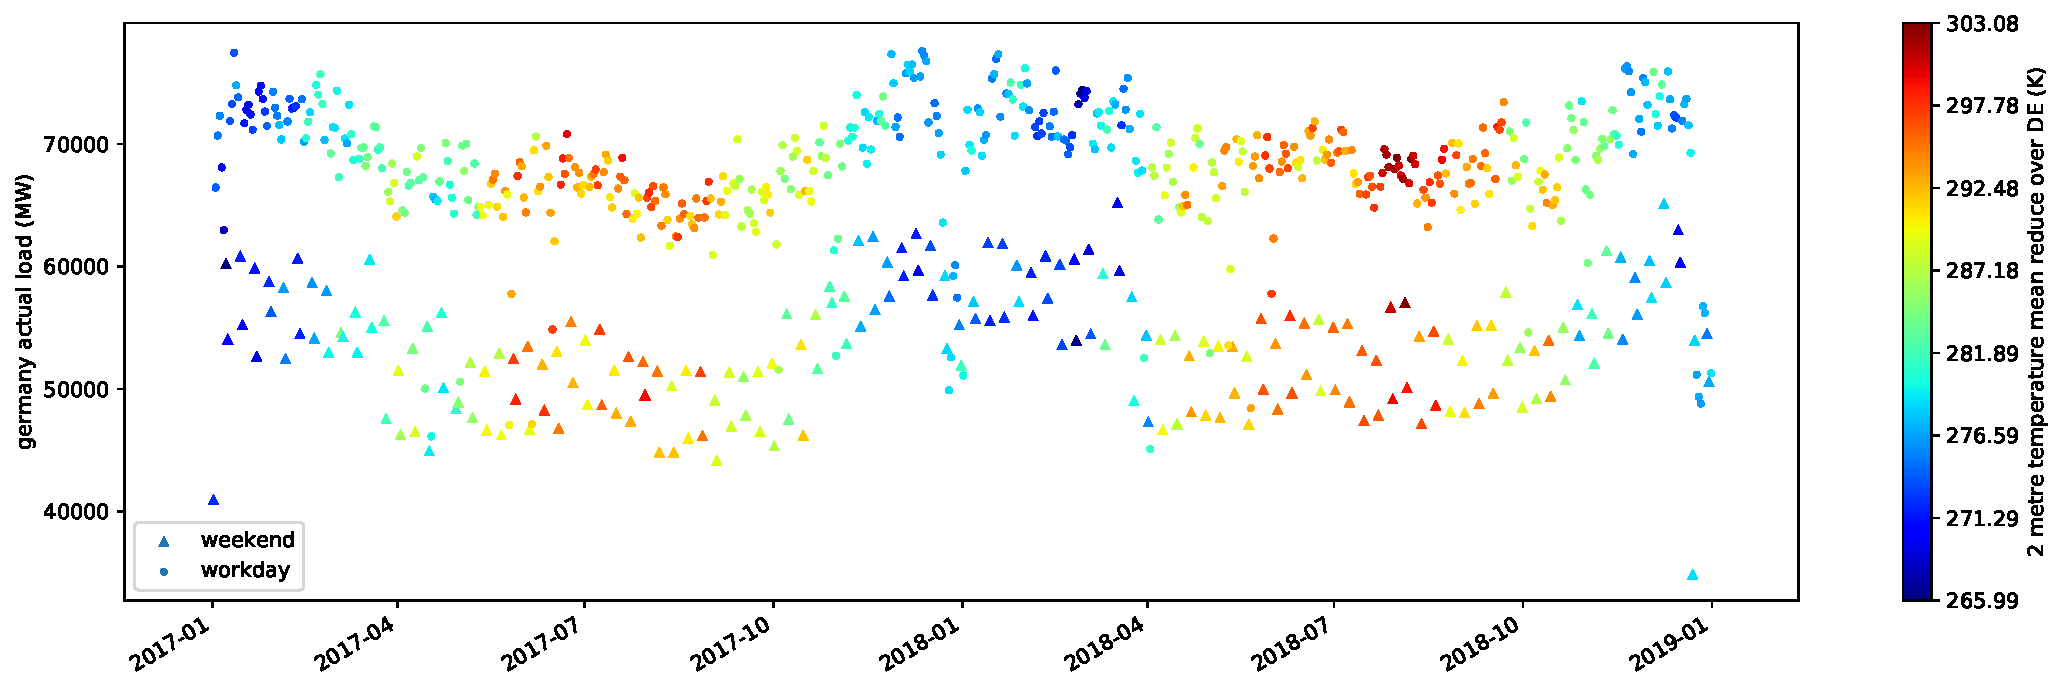
\includegraphics[width=2.9\textwidth,angle=-90,origin=c]{plots/plot_load_time_func/t2m_mean_18A5_2017010112_2018123112_24F}%
		\label{fig:t2m_mean_18A5_2017010112_2018123112_24F}%
	\end{subfigure}%
	\begin{subfigure}{.5\textwidth}
		\centering
		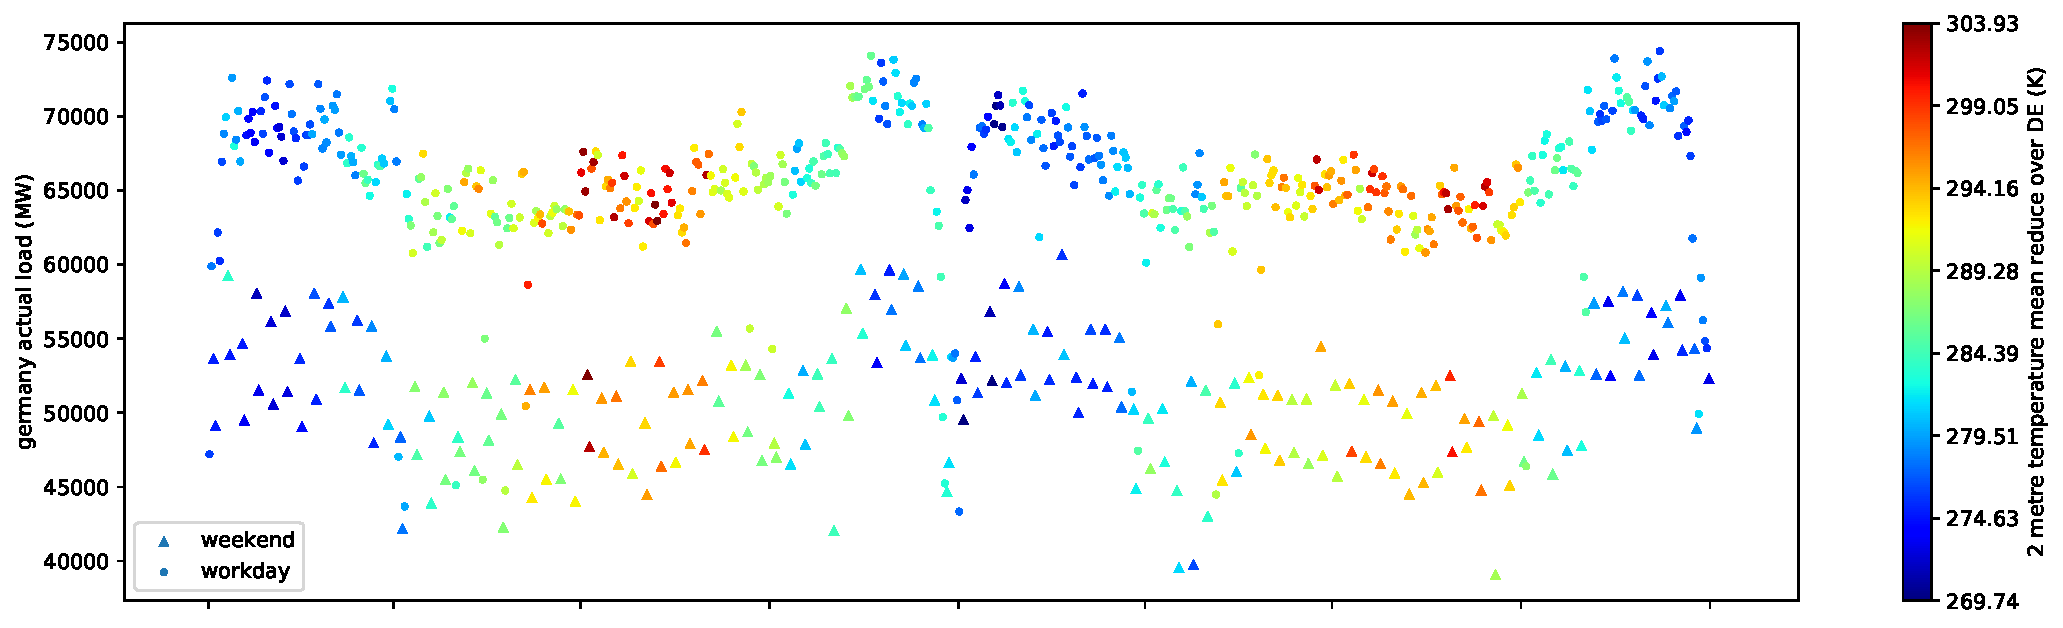
\includegraphics[width=2.9\textwidth,angle=-90,origin=c]{plots/plot_load_time_func/t2m_mean_18A5_2015010112_2016123112_24F}%
		\label{fig:t2m_mean_18A5_2015010112_2016123112_24F}%
	\end{subfigure}
	\caption{Load curve with mean of 2 metre measured temperature in Germany as color from 2015/1/1 to 2018/12/31 with one single point per day at 12 AM UTC time respectively.}
	\label{fig:t2m_mean_18A5_twofold_24F}
\end{figure}


%Describe the data set you are using. Use appropriate visualization (\eg graphs, statistical summaries \etc) to help the reader get to know your data set.

%\Cref{tab:wvars} is an example table. Remember to use full sentences in your caption and explain everything one can see in the table there as well. You can of course also use a simpler format for your table.


\subsection{Population}

For further improvement and in order to figure out important point in the grid, population data for Germany has been  selected from Eurostat\footnote{\url{https://ec.europa.eu/eurostat/data/database}}.\\

\begin{figure}[h!]%
\centering
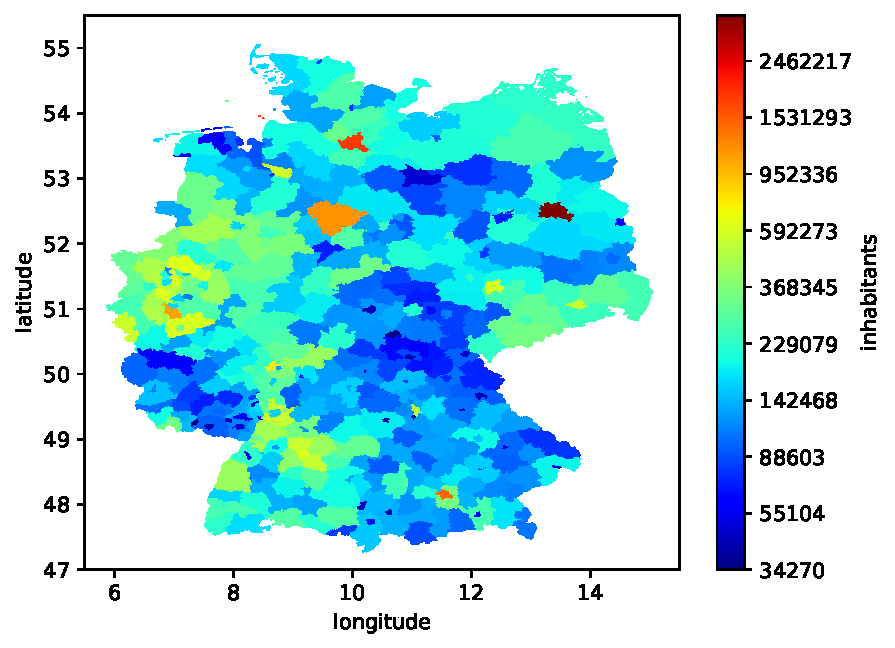
\includegraphics[width=\textwidth]{plots/demo/demo2018_logscale}%
\caption{Population of Germany for each region respectively using a log scale for better distinction.}%
\label{fig:demo2018_logscale}%
\end{figure}


%\begin{table}[h!]%
%\caption{Example table with rotated table heads to save space and two different row colours to ease the readability.}
%\rowcolors{2}{gray!25}{white}
%\centering
%\footnotesize
%\begin{tabular}{lll}
%\toprule \noalign{\smallskip}
%\rottblhead{\tablehead Header 1} & \rottblhead{\tablehead Header 2} & \rottblhead{\tablehead Header 3} \\ \midrule
%entry 1 & entry 2 & entry 3 \\ 
%entry 1 & entry 2 & entry 3 \\ 
%entry 1 & entry 2 & entry 3 \\ 	\bottomrule
%\end{tabular}
%\label{tab:example}
%\end{table}


\section{Programming part}
\label{sec:prog}

\subsection{Programming Language}

For the programming part, Python 3.6+ has been chosen, as there is a variety of libraries to process all used file formats and because it tends to be a time saving language, also for visualization.\\

\subsection{Documentation}

In regard to coding styles, especially when it comes to docstrings, the numpy conventions were used. The three major points for this were first, that it is a popular and often used style, then it is also a visually oriented style which means, that it is easy to read and last it is supported by several (TODO check which, sphinx?!) autodoc tools that create a HTML based documentation from existing source code with docstrings.\\


\section{Preparation}

\begin{figure}[h!]%
	\centering
	\begin{subfigure}{.5\textwidth}
		\centering
		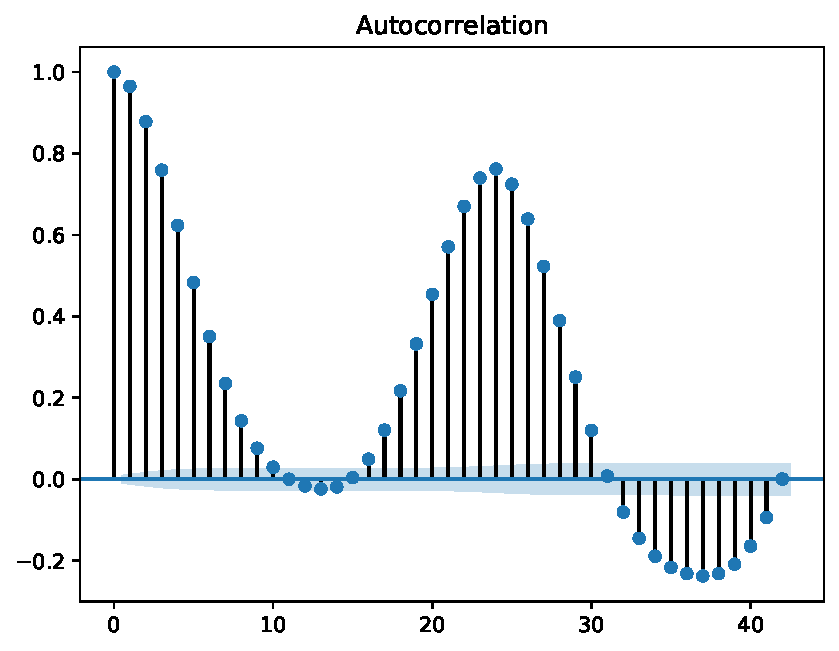
\includegraphics[width=\textwidth]{plots/ACF/load_42lags_ndiff0_hstep1}%
		\caption{}
		\label{fig:acf_load_lags42}%
	\end{subfigure}%
	\begin{subfigure}{.5\textwidth}
		\centering
		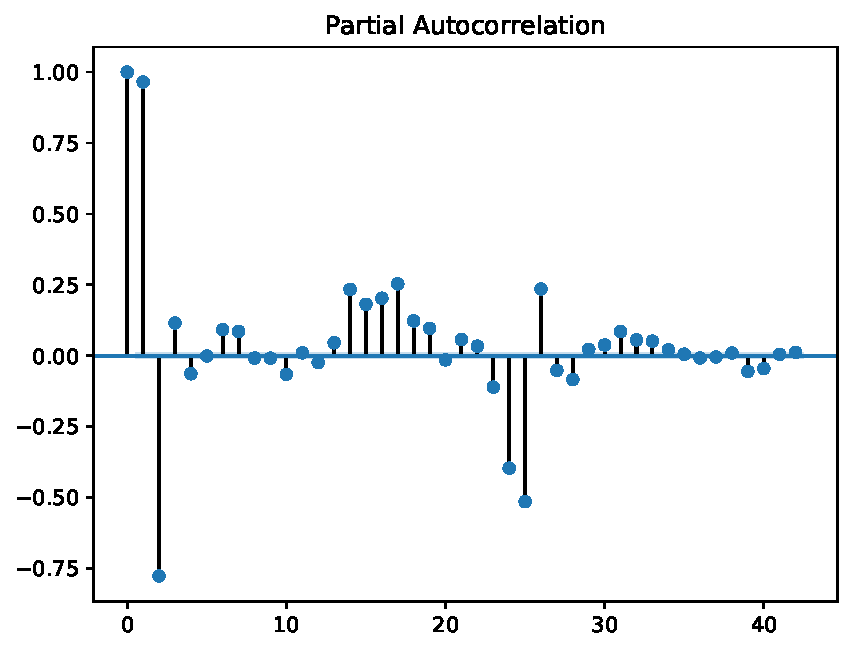
\includegraphics[width=\textwidth]{plots/PACF/load_42lags_ndiff0_hstep1}%
		\caption{}
		\label{fig:pacf_load_lags42}%
	\end{subfigure}
	\caption{Autocorrelation (a) and Partial Autocorrelation (b) plots used to select the order of \acrshort{arma} and \acrshort{armax} models.}
	\label{fig:acf_compare}
\end{figure}


\section{Results}
\label{sec:results}

\subsection{ARMA}

\begin{figure}[h!]%
\centering
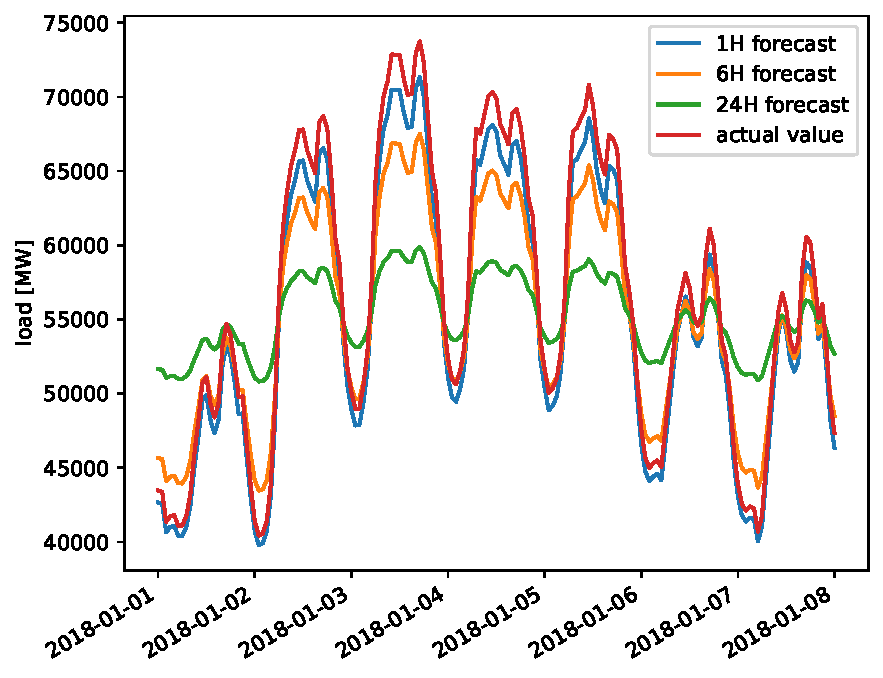
\includegraphics[width=\textwidth]{plots/ARMAfc/ARMA_p1q1_data2015to2018_fcto2018}%
\caption{An example forecast for an ARMA(1,1) using load data from 2015/1/1 to 2018/5/1 forecasting one week for each step 1, 6 and 24 hours respectively.}%
\label{fig:arma_fc}%
\end{figure}

\begin{table}[h!]%
\rowcolors{2}{white}{gray!25}
\centering
\footnotesize
\begin{tabularx}{\linewidth}{lLrrrr}
\tablehead model & \tablehead data & \tablehead\gls{rmse} & \tablehead\gls{mae} & \tablehead\gls{mpe} & \tablehead\gls{mape}\\\hline
ARMA(1,0) & no exogenous data & 67.114 & 66.160 & 0.114 & 0.114\\
ARMAX(1,0) & weekend dummy & 66.913 & 65.963 & 0.114 & 0.114\\
ARMAX(1,0) & t2m mean temperature & 1958.589 & 1930.693 & 3.324 & 3.324\\
ARMAX(1,0) & weekend dummy + t2m mean & 4.417 & 4.157 & -0.008 & 0.008\\
ARMAX(1,0) & t2m data of 10 regions with highest population & 2381.090 & 2347.192 & 4.041 & 4.041\\
ARMAX(1,0) & t2m data of 10 regions with highest population + weekend dummy & 3475.891 & 3426.441 & 5.899 & 5.899\\
\end{tabularx}
\caption{ARMAX results.}
\label{tab:armax_results}
\end{table}


%Describe the results you have obtained using your methods described above. Again use proper visualization methods.
